%----------------------------------------------------------------------------------------
%	PACKAGES AND OTHER DOCUMENT CONFIGURATIONS
%----------------------------------------------------------------------------------------

\documentclass[paper=a4, fontsize=11pt]{scrartcl} % A4 paper and 11pt font size

% ---- Entrada y salida de texto -----

\usepackage[T1]{fontenc} % Use 8-bit encoding that has 256 glyphs
\usepackage[utf8]{inputenc}
%\usepackage{fourier} % Use the Adobe Utopia font for the document - comment this line to return to the LaTeX default

% ---- Idioma --------

\usepackage[spanish, es-tabla]{babel} % Selecciona el español para palabras introducidas automáticamente, p.ej. "septiembre" en la fecha y especifica que se use la palabra Tabla en vez de Cuadro

% ---- Otros paquetes ----
\usepackage{csquotes} %Para permitir el uso de comillas Quotes https://tex.stackexchange.com/questions/36812/isnt-there-any-other-way-of-doing-double-quotes-in-latex-besides
\usepackage[hyphens]{url} % ,href} %para incluir URLs e hipervínculos dentro del texto (aunque hay que instalar href)
\usepackage{hyperref}
\usepackage{color}
\usepackage{graphics,graphicx, floatrow} %para incluir imágenes y notas en las imágenes
\usepackage{graphics,graphicx, float} %para incluir imágenes y colocarlas

\graphicspath {{./img/}}

\usepackage{listings}  %para introducir comandos
\lstset{basicstyle=\ttfamily,
  showstringspaces=false,
  commentstyle=\color{red},
  keywordstyle=\color{blue}
}
% Para hacer tablas comlejas
%\usepackage{multirow}
%\usepackage{threeparttable}

%\usepackage{sectsty} % Allows customizing section commands
%\allsectionsfont{\centering \normalfont\scshape} % Make all sections centered, the default font and small caps

\usepackage{fancyhdr} % Custom headers and footers
\pagestyle{fancyplain} % Makes all pages in the document conform to the custom headers and footers
\fancyhead{} % No page header - if you want one, create it in the same way as the footers below
\fancyfoot[L]{} % Empty left footer
\fancyfoot[C]{} % Empty center footer
\fancyfoot[R]{\thepage} % Page numbering for right footer
\renewcommand{\headrulewidth}{0pt} % Remove header underlines
\renewcommand{\footrulewidth}{0pt} % Remove footer underlines
\setlength{\headheight}{13.6pt} % Customize the height of the header

\setlength\parindent{0pt} % Removes all indentation from paragraphs - comment this line for an assignment with lots of text

\newcommand{\horrule}[1]{\rule{\linewidth}{#1}} % Create horizontal rule command with 1 argument of height


%----------------------------------------------------------------------------------------
%	TÍTULO Y DATOS DEL ALUMNO
%----------------------------------------------------------------------------------------

\title{	
\normalfont \normalsize 
\textsc{\textbf{Ingeniería de Servidores (2021-2022)} \\ Grado en Ingeniería Informática \\ Universidad de Granada} \\ [25pt] % Your university, school and/or department name(s)
\horrule{0.5pt} \\[0.4cm] % Thin top horizontal rule
\huge Memoria Práctica 4 \\ % The assignment title
\horrule{2pt} \\[0.5cm] % Thick bottom horizontal rule
}

\author{Adrián Acosa Sánchez} % Nombre y apellidos

\date{\normalsize\today} % Incluye la fecha actual

%----------------------------------------------------------------------------------------
% DOCUMENTO
%----------------------------------------------------------------------------------------

\begin{document}

\maketitle % Muestra el Título

\newpage %inserta un salto de página

\tableofcontents % para generar el índice de contenidos
 
\newpage

%----------------------------------------------------------------------------------------
%	Cuestión 1
%----------------------------------------------------------------------------------------

\section{Ejercicio 1: Phoronix}

\subsection{Instalación de Phoronix}

\subsubsection{Instalación de Phoronix en Ubuntu}

Para descargar Phoronix en ubuntu tenemos que usar el comando wget para descargarlo de la página oficial:

\begin{figure}[H]
    \centering
    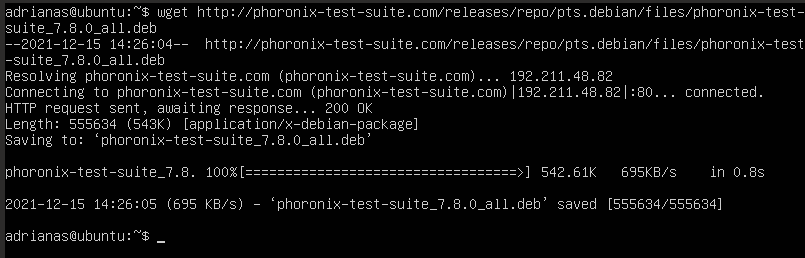
\includegraphics[scale=0.5]{ubuntu/img1}
    \caption{Ejecución del comando wget para descargar Phoronix}
\end{figure}

Para poder instalar archivos $.deb$ tenemos que antes instalar una herramienta llamada $gdebi-core$ de los repositorios oficiales de Ubuntu:

\begin{figure}[H]
    \centering
    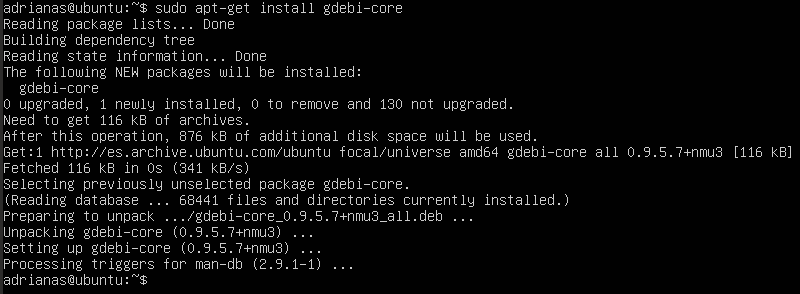
\includegraphics[scale=0.5]{ubuntu/img2}
    \caption{Instalacion de la herramienta para instalar paquetes $.deb$}
\end{figure}

Una vez tenemos el archivo $.deb$ y la herramienta que nos permite instalar archivos con esta extensión, procedemos a instalar el paquete de phoronix:

\begin{lstlisting}[language=bash]
    sudo gdebi phoronix-test-suite_7.8.0_all.deb 
\end{lstlisting}

\subsubsection{Lista de los Benchmarks disponibles en Phoronix (Ubuntu)}

Para poder ver la lista de benchmarks disponibles con el paquete phoronix, ejecutamos el siguiente comando:

\begin{lstlisting}[language=bash]
    phoronix-test-suite list-tests
\end{lstlisting}

\begin{figure}[H]
    \centering
    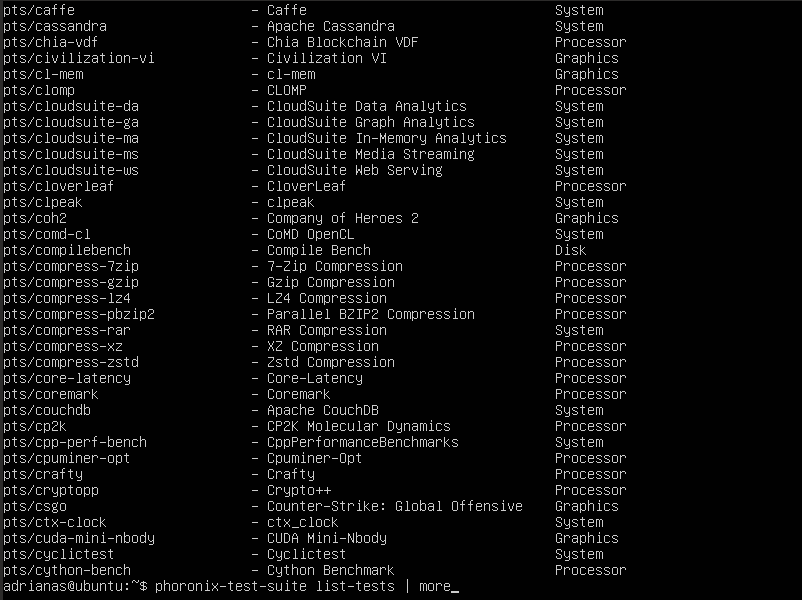
\includegraphics[scale=0.5]{ubuntu/img7}
    \caption{Listado de todos los benchmark proporcionados por Phoronix}
\end{figure}

\newpage
\subsubsection{Ejecución de Benchmarks en Ubuntu}

Para poder ejecutar un benchmark de los proporcionados por Phoronix, tenemos que ejecutar el siguiente comando:

\begin{lstlisting}[language=bash]
    phoronix-test-suite run pts/coremark
\end{lstlisting}

Cuando ejecutemos un benchmark, si este no está instalado te pedirá que lo instales. Así que le decimos que sí como en la siguiente imagen:

\begin{figure}[H]
    \centering
    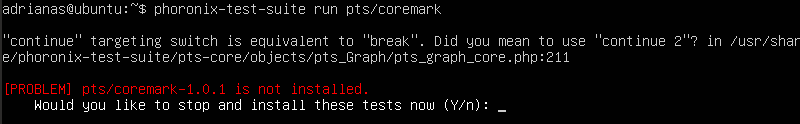
\includegraphics[scale=0.5]{ubuntu/img9}
    \caption{Ejecución de un benchmark en Ubuntu}
\end{figure}

También nos pedirá que instalemos sus dependencias necesarias para la correcta ejecución del benchmark:

\begin{figure}[H]
    \centering
    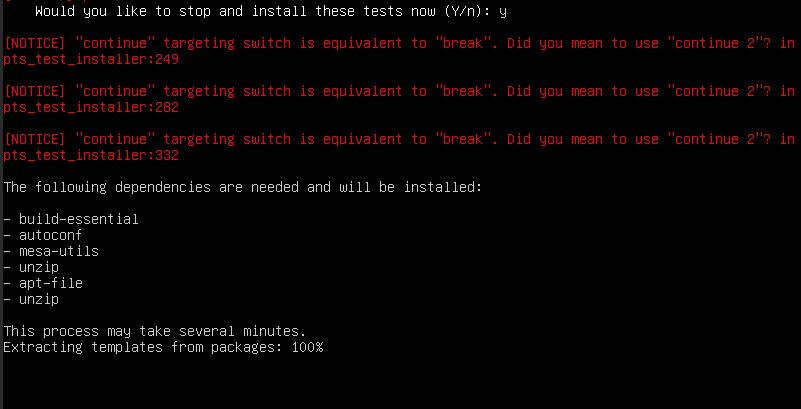
\includegraphics[scale=0.5]{ubuntu/img10}
    \caption{Dependencias del benchmark}
\end{figure}
    
Una vez instalado nos enseñará información sobre nuestro hardware y empezará a preguntarnos si queremos guardar los resultados cuando termine de ejecutar dicho benchmark. En mi caso le digo que sí y le pongo un nombre (la descripción la dejo vacía porque es una prueba):

\begin{figure}[H]
    \centering
    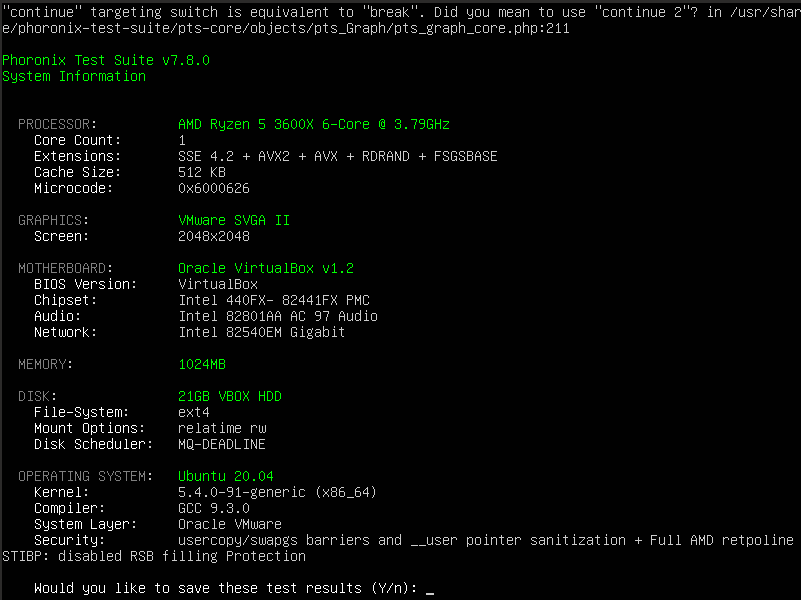
\includegraphics[scale=0.5]{ubuntu/img11}
    \caption{Información adicional sobre la ejecución del Benchmark}
\end{figure}

Una vez terminamos de completar toda la información pedida para la ejecución del benchmark, se empezará a ejecutar y cuando termine nos preguntará si queremos ver los resultados:

\begin{figure}[H]
    \centering
    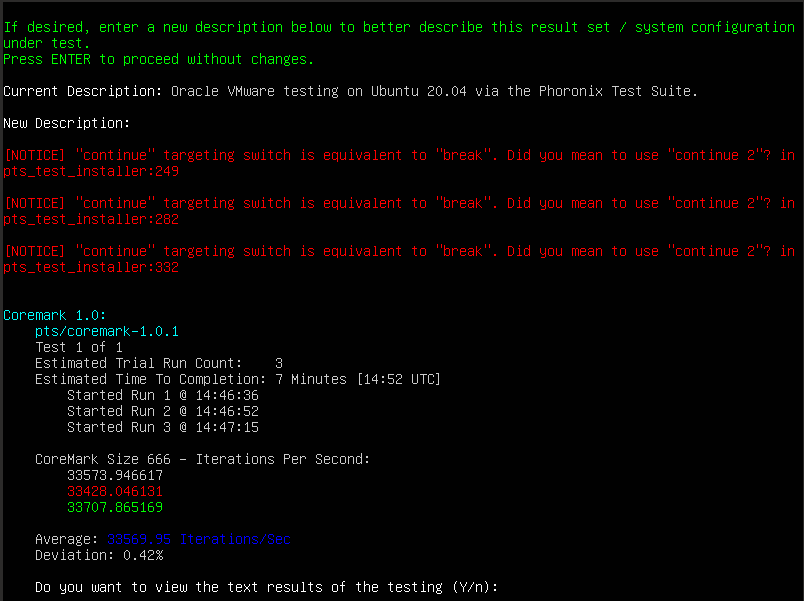
\includegraphics[scale=0.5]{ubuntu/img12}
    \caption{Resultados del Benchmark}
\end{figure}

\begin{figure}[H]
    \centering
    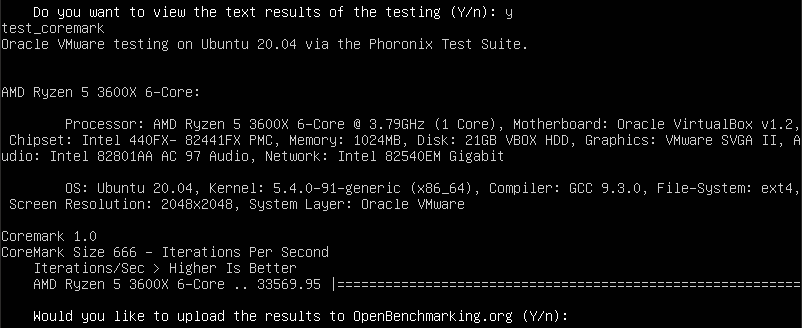
\includegraphics[scale=0.5]{ubuntu/img13}
    \caption{Resultados numéricos del Benchmark}
\end{figure}

Nos pregunta también si queremos verlo en una página web donde aparecen los datos más ordenados. En esa página sale la siguiente información:

\begin{figure}[H]
    \centering
    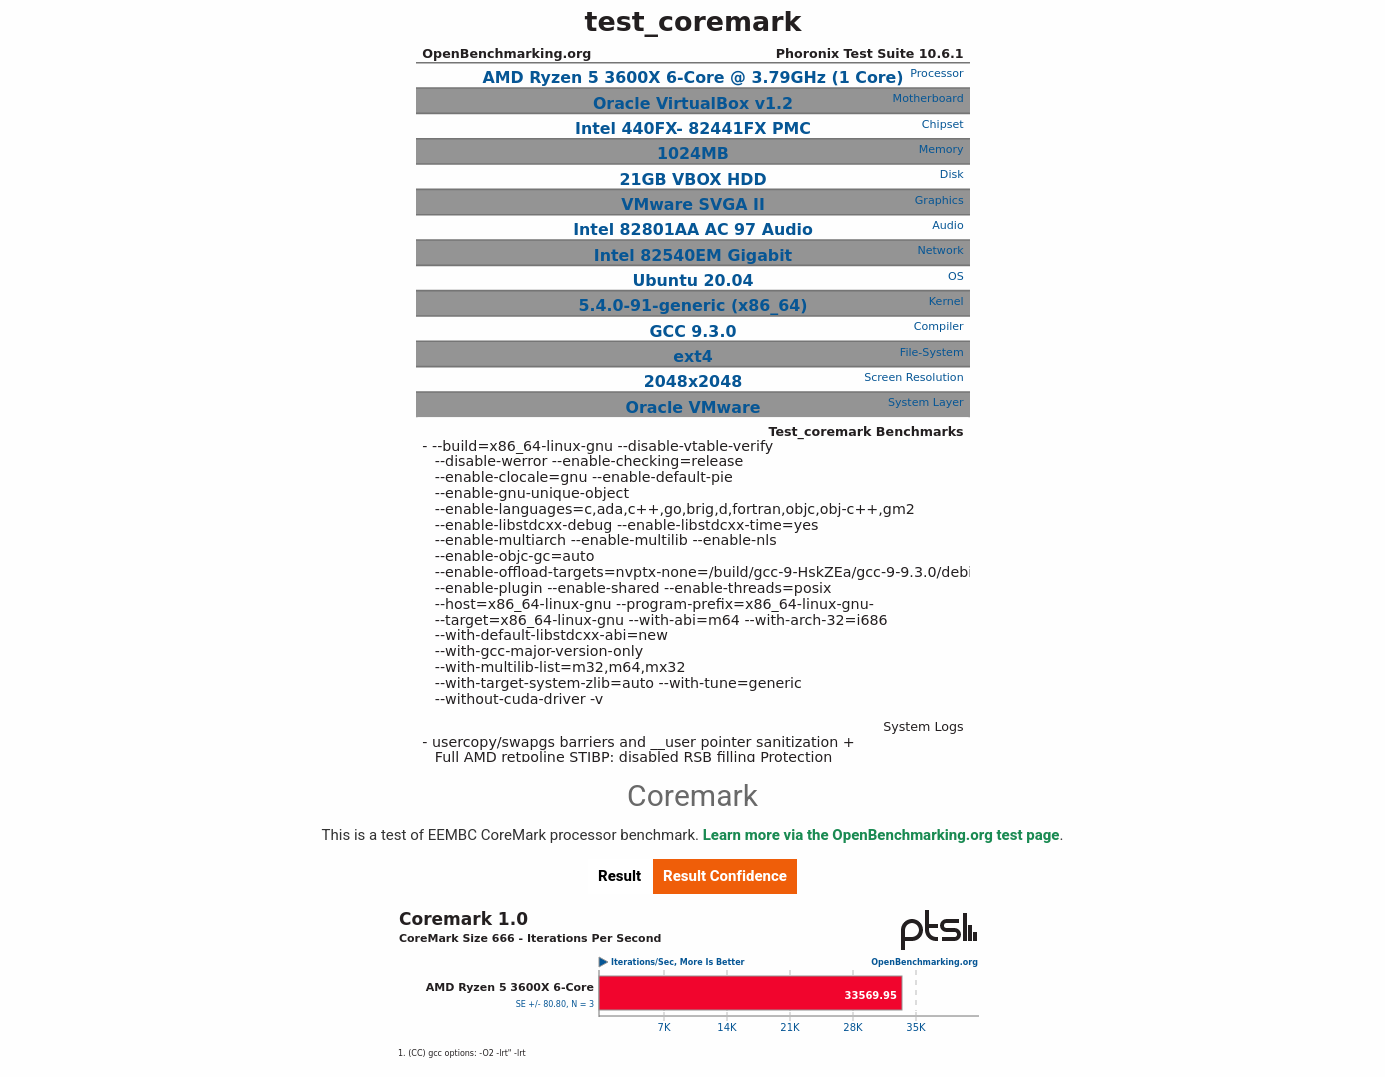
\includegraphics[scale=0.3]{ubuntu/test-coremark}
    \caption{Resultados del Benchmark en página web}
\end{figure}

\newpage
Ejecutamos ahora un benchmark de git:

\begin{figure}[H]
    \centering
    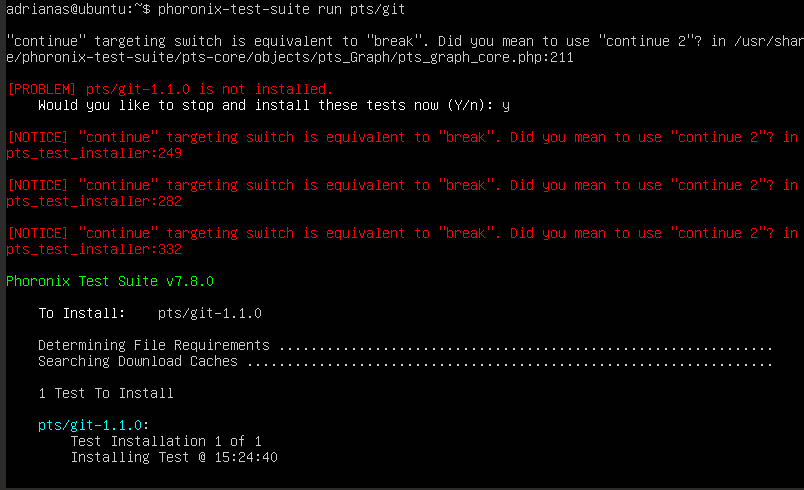
\includegraphics[scale=0.35]{ubuntu/img14}
    \caption{Instalación del Benchmark de Git}
\end{figure}

\begin{figure}[H]
    \centering
    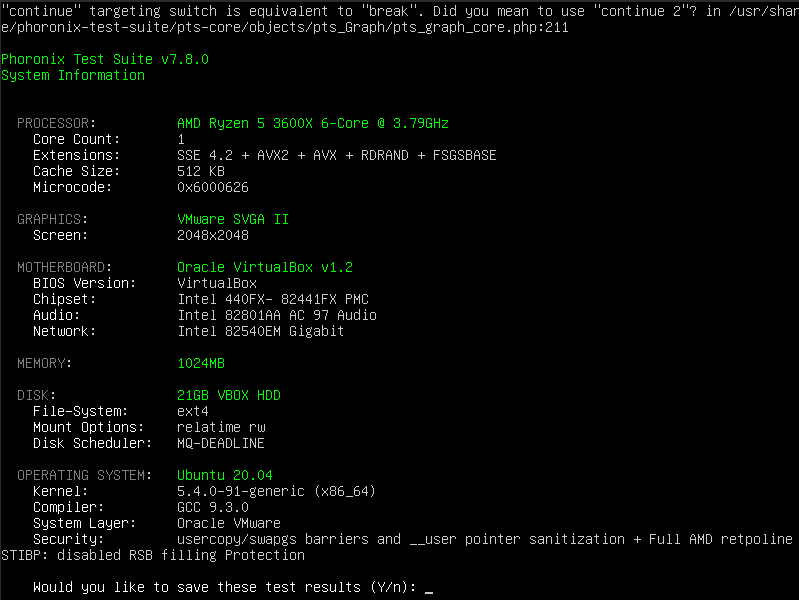
\includegraphics[scale=0.35]{ubuntu/img15}
    \caption{Ejecución del Benchmark de Git}
\end{figure}

\begin{figure}[H]
    \centering
    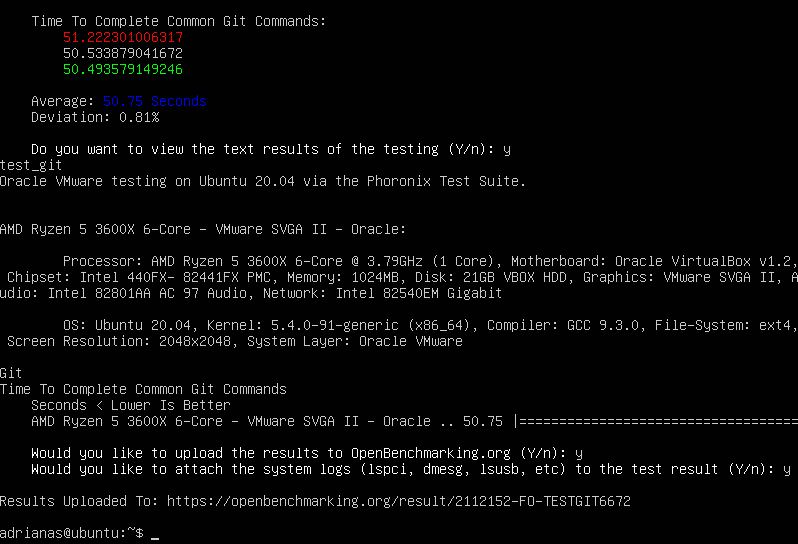
\includegraphics[scale=0.35]{ubuntu/img16}
    \caption{Resultados del Benchmark de Git}
\end{figure}

\begin{figure}[H]
    \centering
    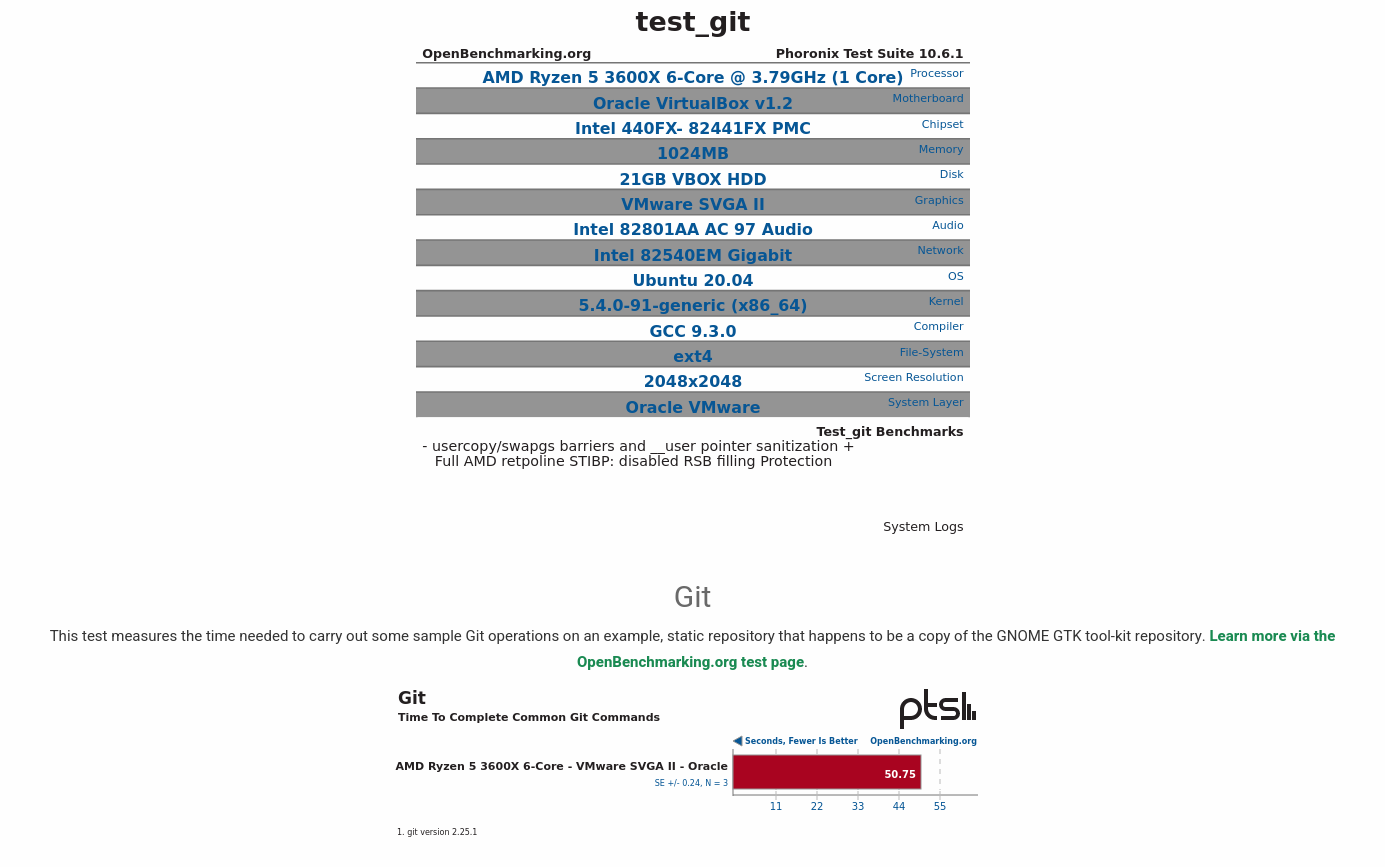
\includegraphics[scale=0.3]{ubuntu/test-git}
    \caption{Resultados de Benchmark de Git en página web}
\end{figure}

\newpage
\subsubsection{Instalación de Phoronix en CentOS}

La instalación en CentOS es muy parecida a la de Ubuntu. Comenzamos por instalar los paquetes que aparecen en la siguiente imagen:

\begin{figure}[H]
    \centering
    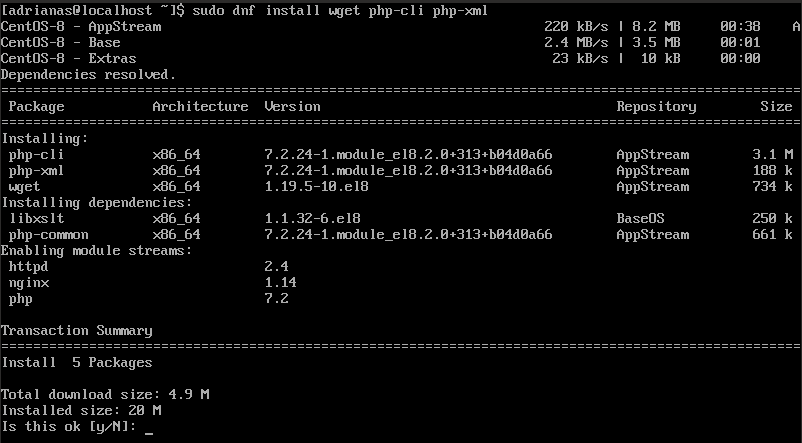
\includegraphics[scale=0.5]{centos/img1}
    \caption{Instalación de paquetes necesarios para Phoronix}
\end{figure}

Tras esto tendremos que descargar el paquete de phoronix con wget desde su repositorio oficial:

\begin{figure}[H]
    \centering
    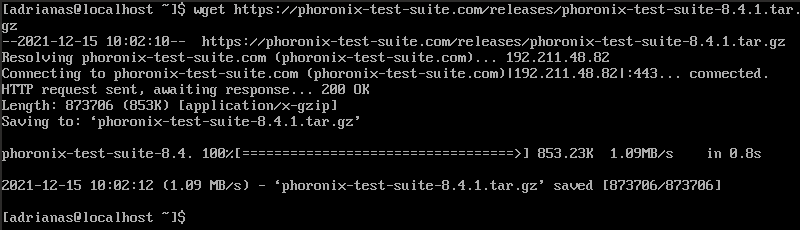
\includegraphics[scale=0.5]{centos/img2}
    \caption{Descarga de Phoronix de su repositorio oficial}
\end{figure}

\newpage
Lo descomprimimos y ejecutamos el archivo install-sh contenido en la carpeta de Phoronix:

\begin{figure}[H]
    \centering
    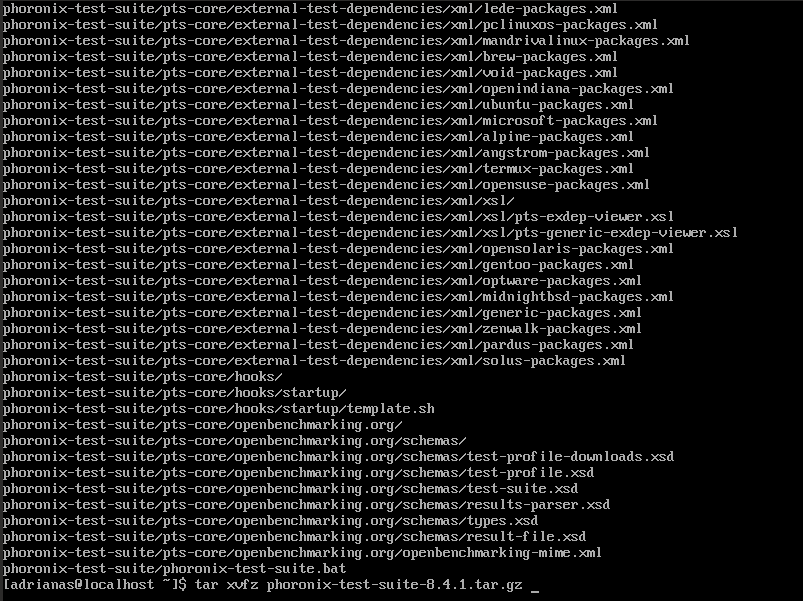
\includegraphics[scale=0.5]{centos/img3}
    \caption{Descompresión del archivo descargado de Phoronix}
\end{figure}

\begin{figure}[H]
    \centering
    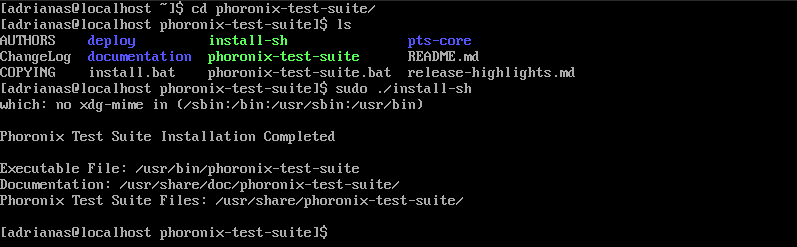
\includegraphics[scale=0.5]{centos/img4}
    \caption{Ejecución del instalador de Phoronix}
\end{figure}

\newpage
\subsubsection{Lista de los Benchmarks disponibles en Phoronix (CentOS)}

Una vez ejecutado todo lo anterior procedemos a listar todos los Benchmarks disponibles en CentOS

\begin{figure}[H]
    \centering
    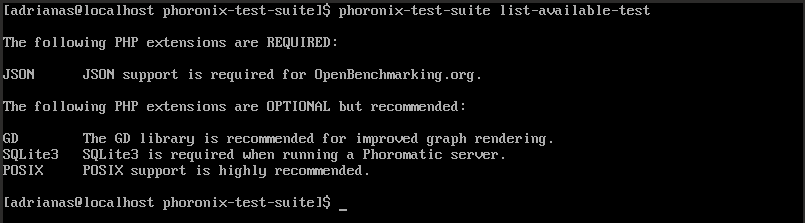
\includegraphics[scale=0.5]{centos/img5}
    \caption{Error de listados Benchmarks disponibles de Phoronix en CentOS}
\end{figure}

Pero nos da un error ya que no tenemos todas las dependencias necesarias para ejecutarlos. Luego instalamos las dependencias como aparece en la siguiente imagen:

\begin{figure}[H]
    \centering
    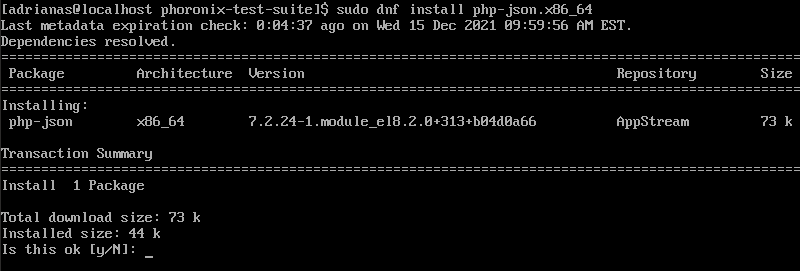
\includegraphics[scale=0.5]{centos/img6}
    \caption{Instalación de dependencias necesarias}
\end{figure}

Una vez hecho esto ya podremos listar todos los Benchmarks disponibles con la siguiente orden:

\begin{lstlisting}[language=bash]
    phoronix-test-suite list-available-tests
\end{lstlisting}

\newpage
\subsubsection{Ejecución de Benchmarks en centos}

Para comparar los rendimientos entre ambos sistemas operativos voy a eecutar los mismos test que en Ubuntu. En las siguientes fotos aparecen los datos de ambos Benchmarks:

En mi caso, para poder ejecutar el benchmark coremark tuve problemas de dependencias para poder ejecutarlo. Así que tuve que habilitar los PowerTools de los repositorios de CentOS para poder instalar dichas dependencias:

\begin{figure}[H]
    \centering
    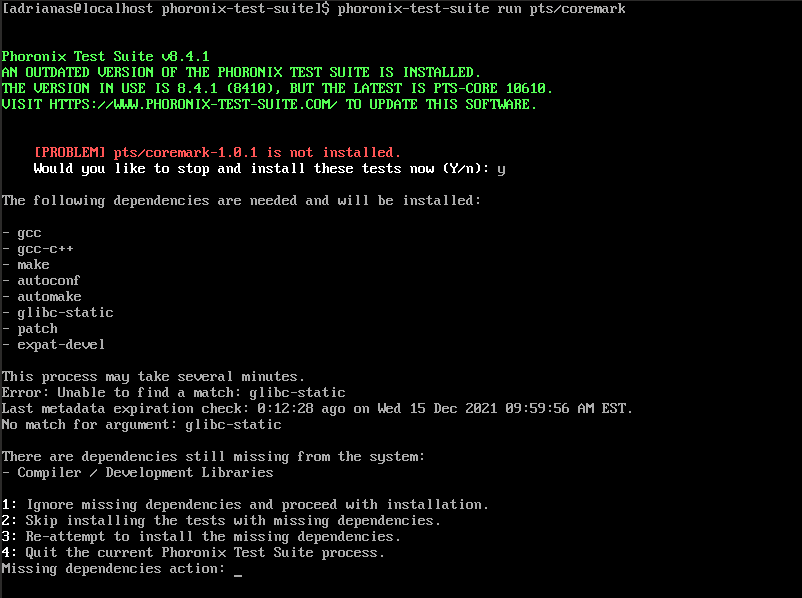
\includegraphics[scale=0.5]{centos/img9}
    \caption{Dependencias de pts/coremark}
\end{figure}

\begin{figure}[H]
    \centering
    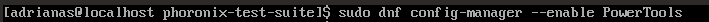
\includegraphics[scale=0.5]{centos/img10}
    \caption{Habilitando los PowerTools de yum}
\end{figure}

\newpage
Una vez hecho esto, comenzamos con la ejecución de ambos benchmarks. En primer lugar el benchmark de coremark:

\begin{figure}[H]
    \centering
    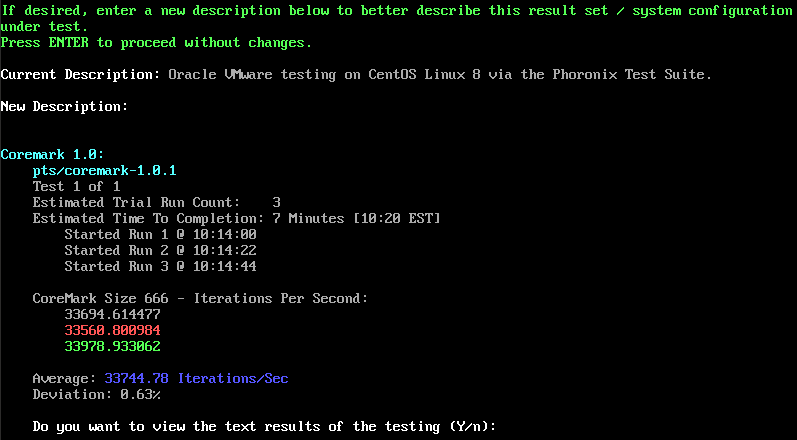
\includegraphics[scale=0.5]{centos/img12}
    \caption{Ejecución del benchmark coremark}
\end{figure}

\begin{figure}[H]
    \centering
    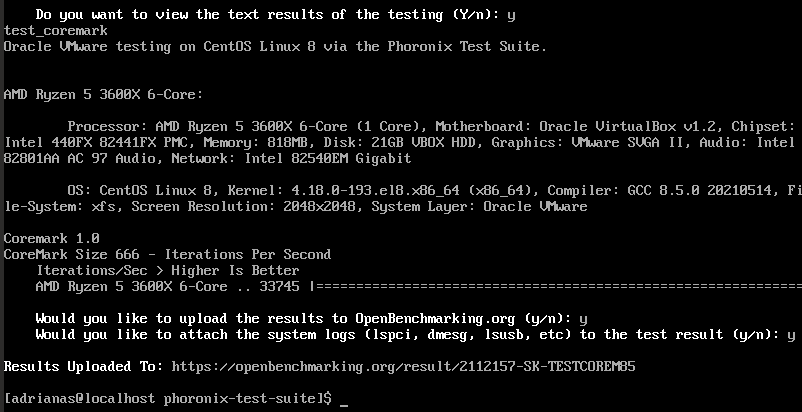
\includegraphics[scale=0.5]{centos/img14}
    \caption{Resultados del benchmark coremark}
\end{figure}

\begin{figure}[H]
    \centering
    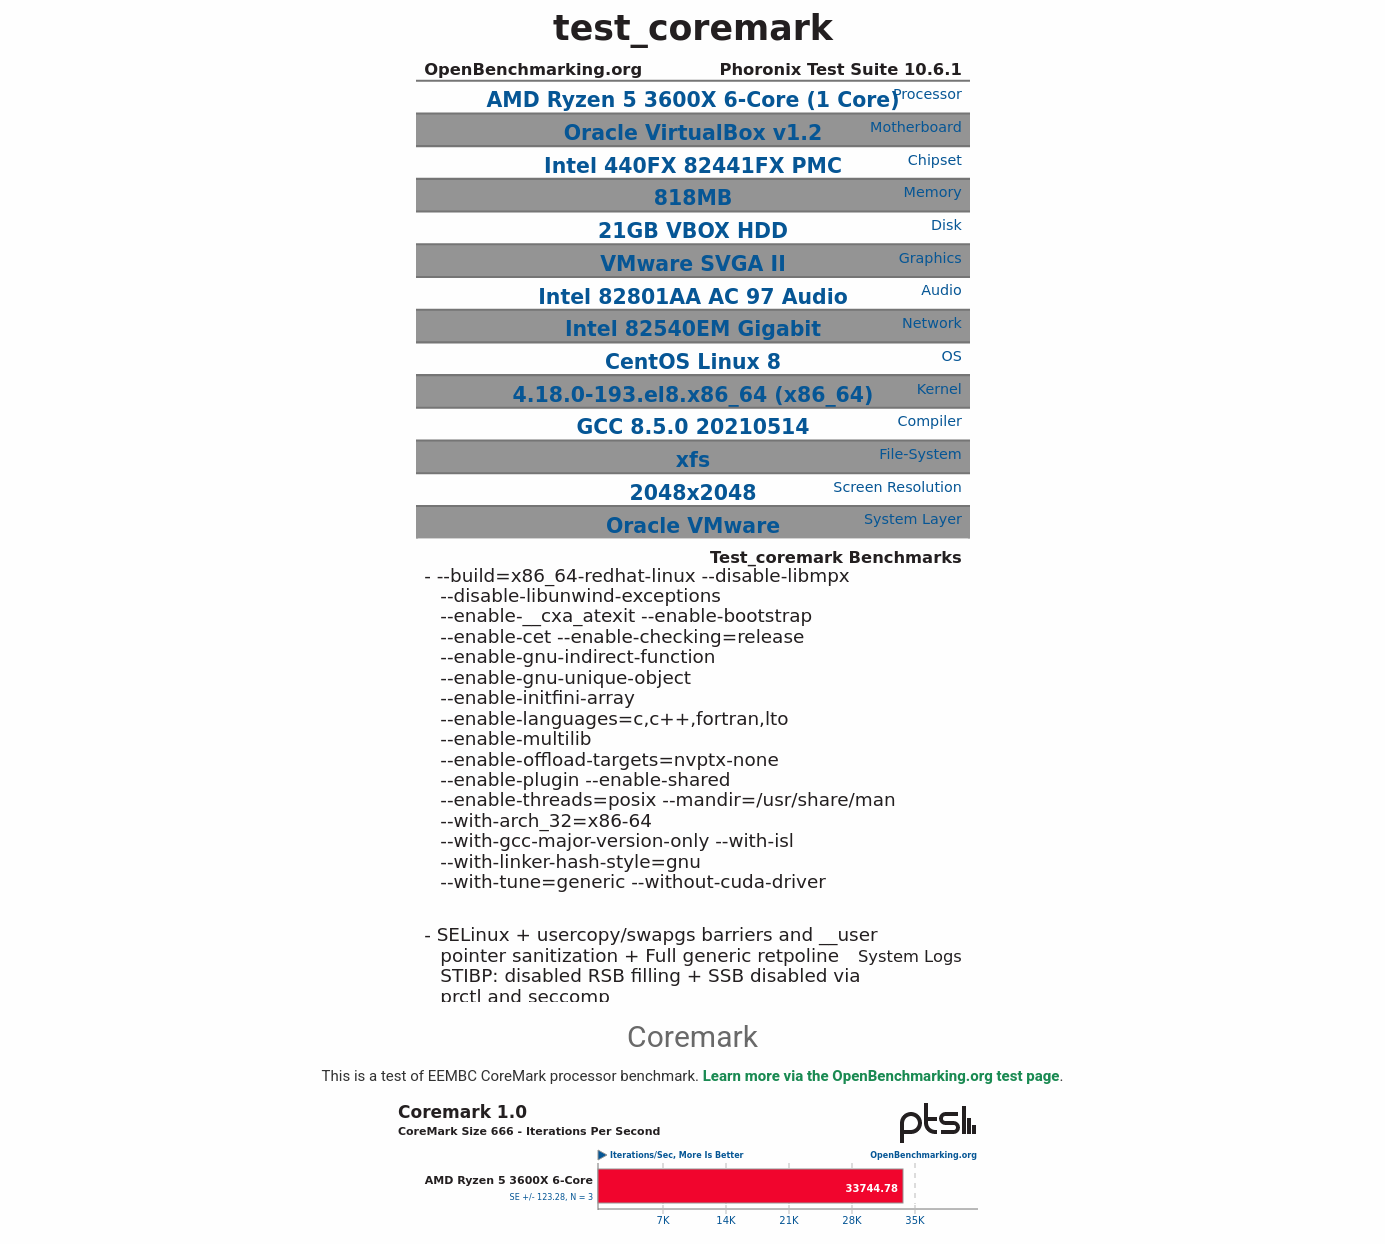
\includegraphics[scale=0.3]{centos/test-coremark}
    \caption{Resultados de la página web del test coremark}
\end{figure}

\newpage
Y ahora la ejecución del benchmark de Git:

\begin{figure}[H]
    \centering
    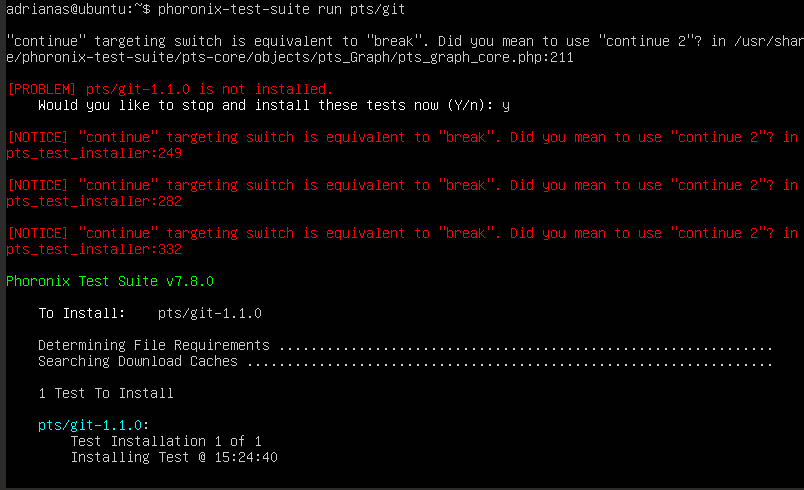
\includegraphics[scale=0.4]{centos/img18}
    \caption{Instalación del benchmark de Git}
\end{figure}

\begin{figure}[H]
    \centering
    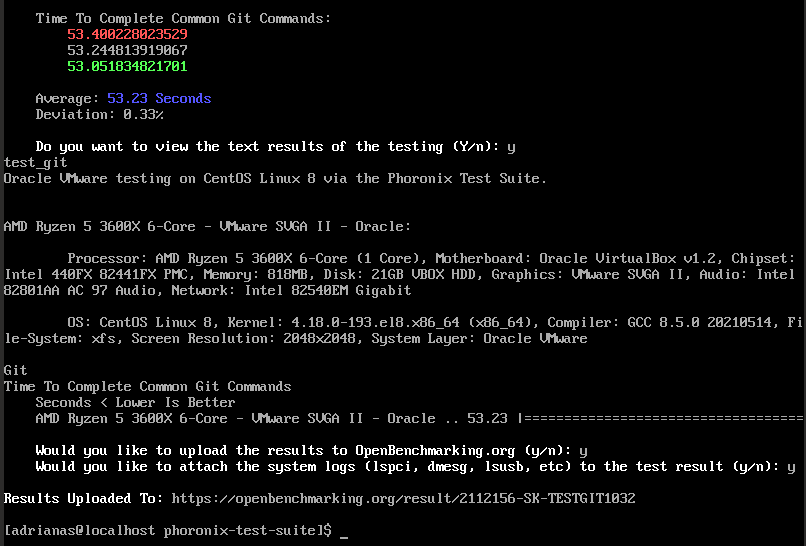
\includegraphics[scale=0.4]{centos/img21}
    \caption{Ejecución del benchmark de Git}
\end{figure}

\begin{figure}[H]
    \centering
    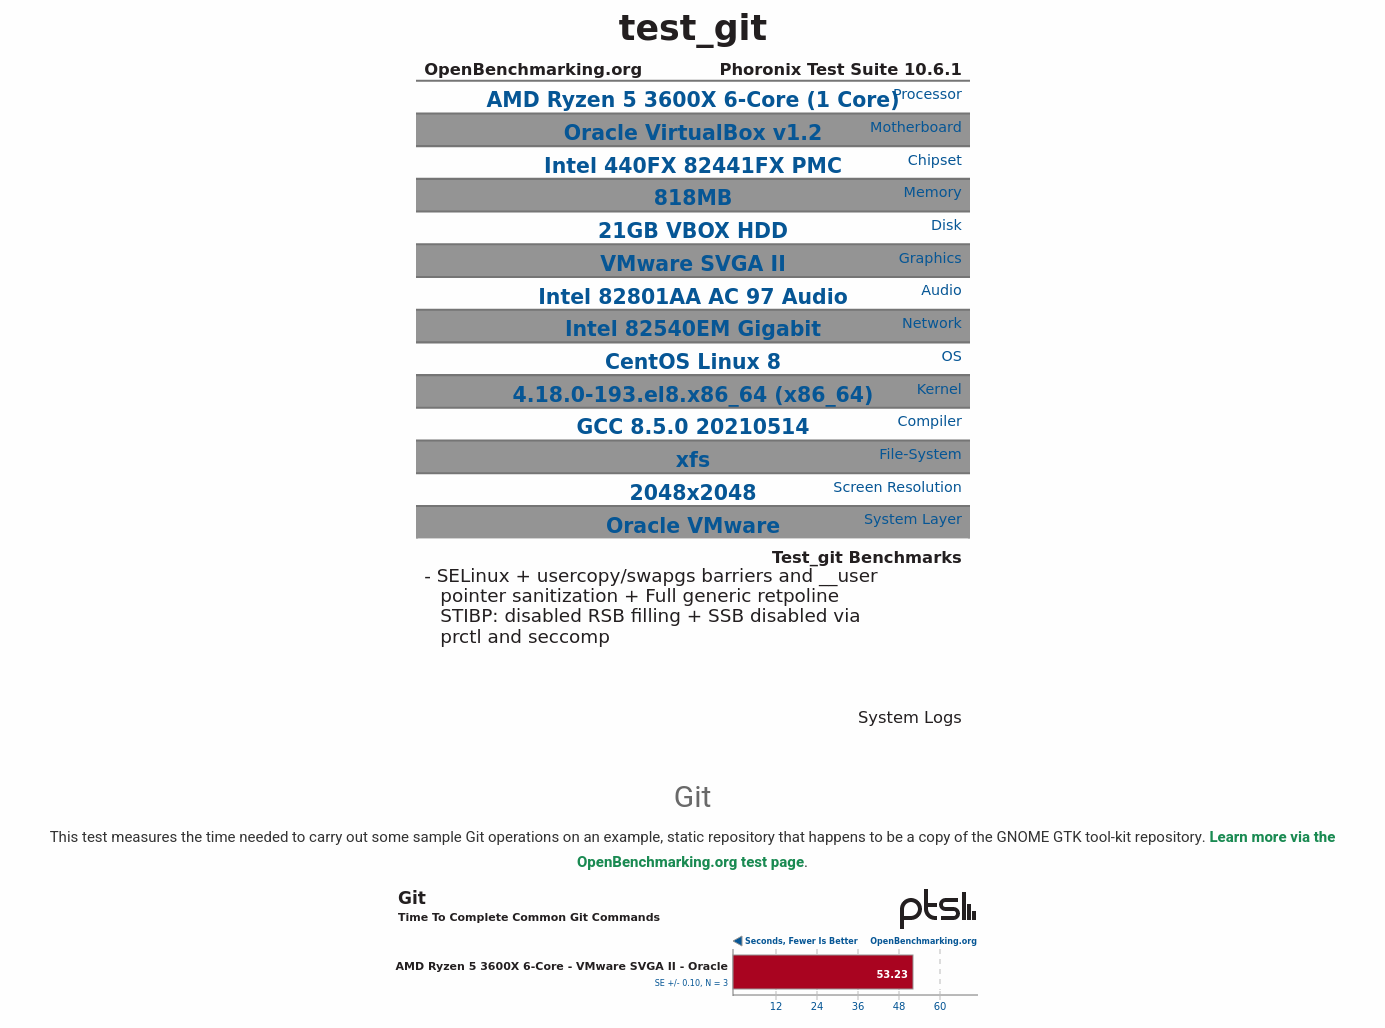
\includegraphics[scale=0.3]{centos/test-git}
    \caption{Resultados de la página web del test Git}
\end{figure}

Los resultados para coremark son para CentOS 33745 y para Ubuntu 33569.
Los resultados para Git son para CentOS 53.23 y para Ubuntu 50.75.
Como podemos ver, no hay una diferencia clara entre ambos sistemas ya que los valores de los benchmarks tienen diferencias de muy poca puntuación (tiene sentido ya que se ejecutan sobre el mismo Host).


%----------------------------------------------------------------------------------------
%	Cuestión 2
%----------------------------------------------------------------------------------------

\newpage
\section{Ejercicio 2: JMeter}

\subsection{Instalación de JMeter (Ubuntu)}

Antes de instalar JMeter tenemos que instalar docker y docker-compose para poder descargar el repositorio que se proporciona:

\begin{lstlisting}[language=bash]
    sudo apt-get install docker docker-compose
\end{lstlisting}

Ahora vamos a descargar el repositorio de JMeter proporcionado para hacer la práctica con el siguiente comando:

\begin{figure}[H]
    \centering
    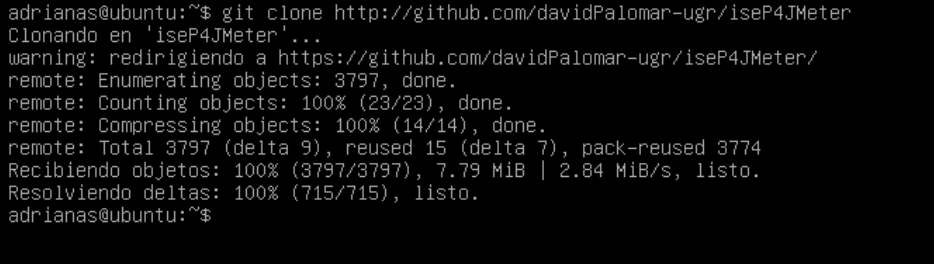
\includegraphics[scale=0.45]{JMeter/img2}
    \caption{Descarga de la carpeta con JMeter}
\end{figure}

Una vez descargada la carpeta, iniciamos el servicio con el comando:

\begin{lstlisting}[language=bash]
    sudo docker-compose up
    sudo docker-compose down
\end{lstlisting}

up para levanatar el servicio y down para pararlo. La ejecución de docker ensucia mucho la pantalla con muchos outputs. Para que no 
que no imprima nada por pantalla, ejecutamos el siguiente comando:

\begin{figure}[H]
    \centering
    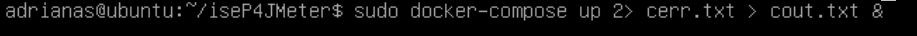
\includegraphics[scale=0.5]{JMeter/img7}
    \caption{Levantar el servicio sin outputs}
\end{figure}

La primera vez tardará un rato ya que tendrá que descargar todos los contenedores. Una vez termine, tendremos que habilitar el puerto 3000 ya que el servicio lo requiere.
Esto, como ya sabemos, lo haremos con el comando:

\begin{lstlisting}[language=bash]
    ufw enable
    ufw allow 3000/tcp    
\end{lstlisting}

Para ver si todo se ha iniciado correctamente, lo comprobamos en un navegador poniendo la IP de nuestro servidor seguido del puerto 3000 y tendría que salir un resultado como el siguiente:

\begin{figure}[H]
    \centering
    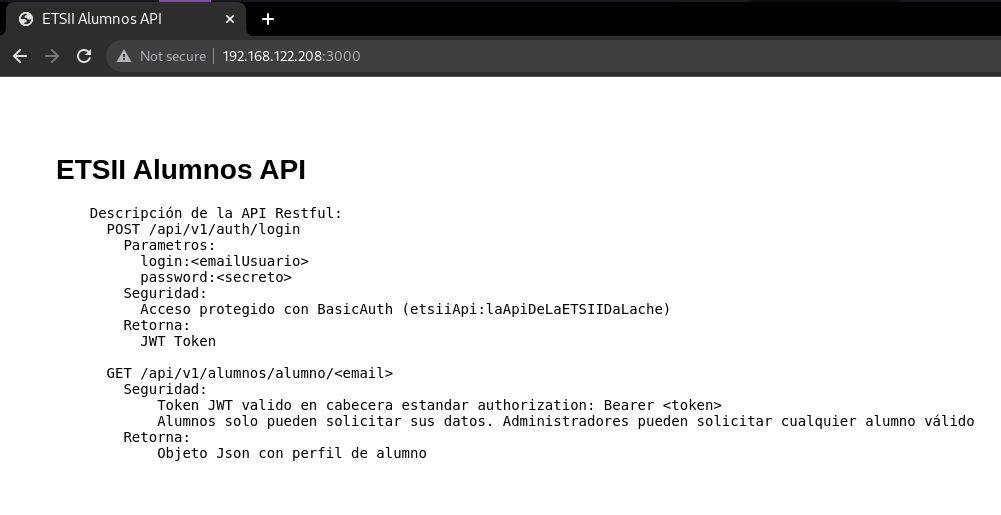
\includegraphics[scale=0.4]{JMeter/img6}
    \caption{Pantalla de inicio del servicio}
\end{figure}

\subsection{Instalación de JMeter en nuestro Host}

El único requisito que tiene JMeter para permitir su ejecución es tener Java instalado y lo podemos comprobar con la ejecución del comando:

\begin{lstlisting}[language=bash]
    java --version
\end{lstlisting}

Una vez comprobamos que tenemos Java instalado, nos vamos a la página oficial de JMeter y lo descargamos. Al descomprimirlo nos vamos a su carpeta y ejecutamos el archivo cuyo nombre es ApacheJMeter.jar:

\begin{figure}[H]
    \centering
    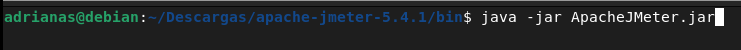
\includegraphics[scale=0.5]{JMeter/img11}
    \caption{Ejecución con Java de JMeter.}
\end{figure}

Al abrirlo nos aparecerá una ventana como la siguiente:

\begin{figure}[H]
    \centering
    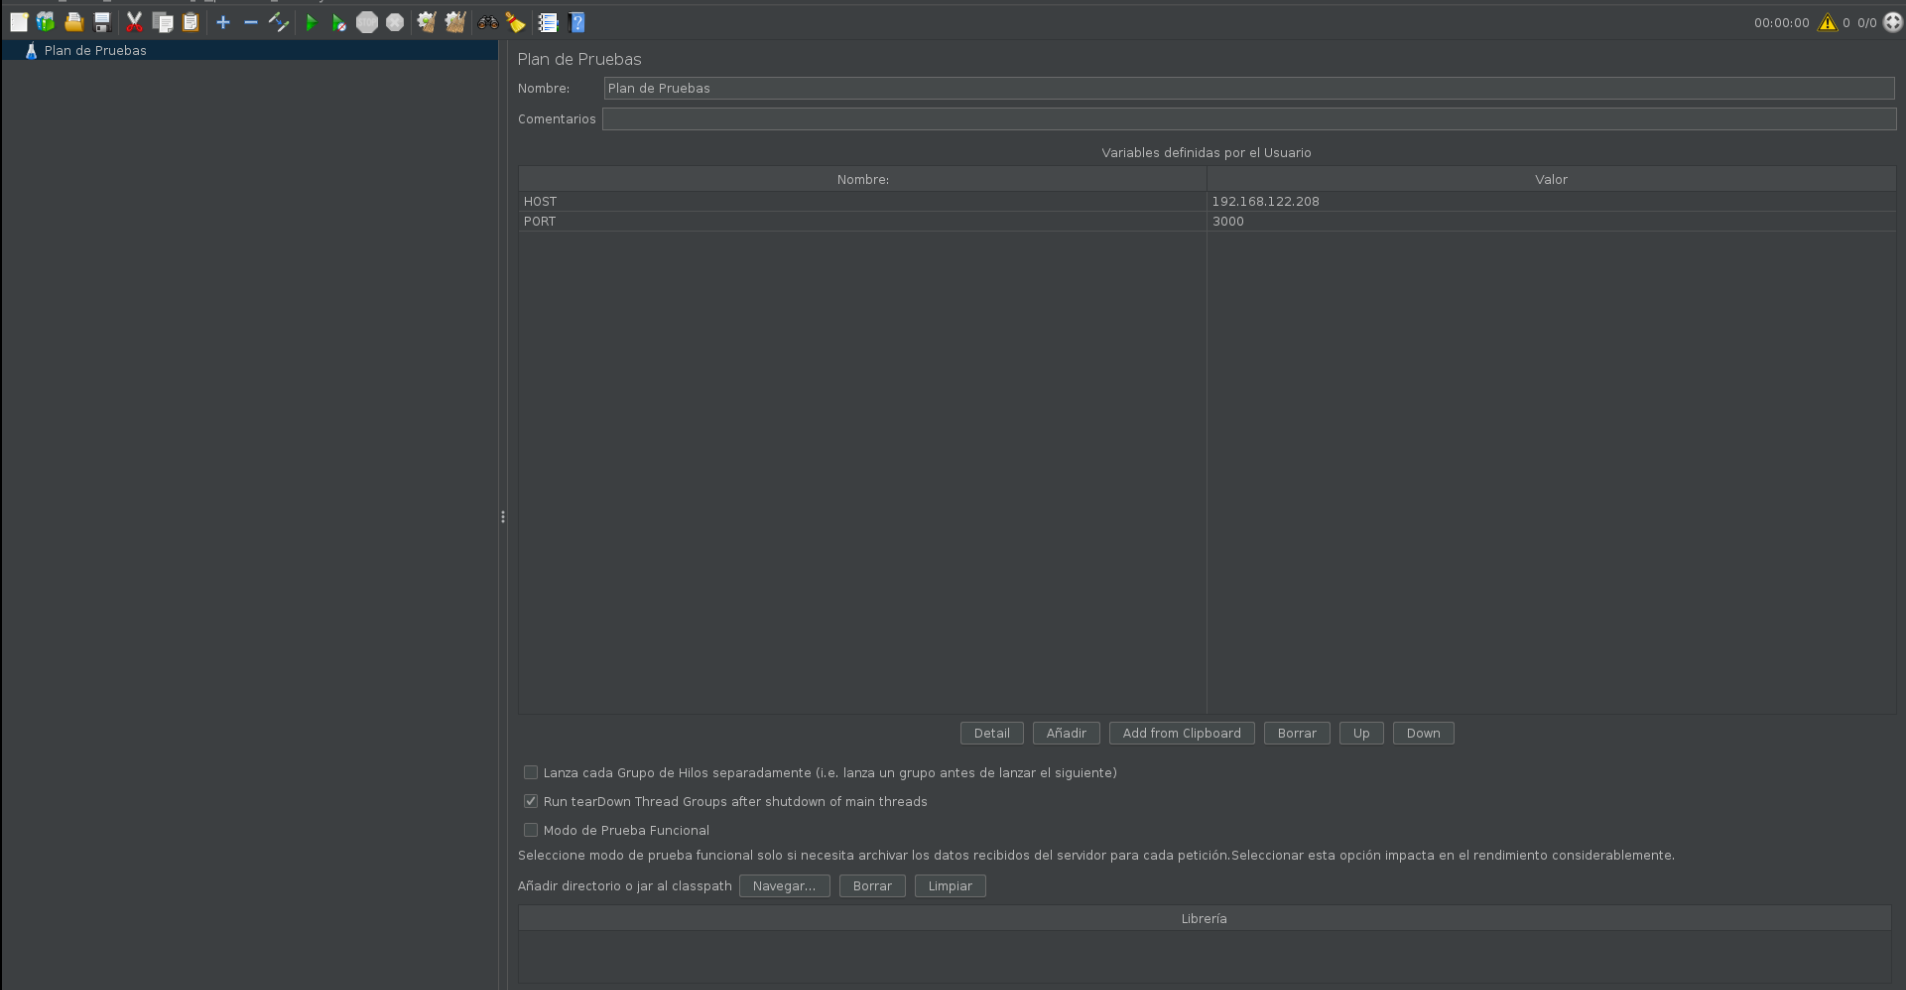
\includegraphics[scale=0.25]{JMeter/img12}
    \caption{Pantalla inicial de JMeter}
\end{figure}

\subsubsection{Parametrizar el Host y el Puerto en el Test Plan}

Para lograr parametrizar el Host y el Puerto tenemos que añadir al nodo principal los datos de nuestra IP y el Puerto:

\begin{figure}[H]
    \centering
    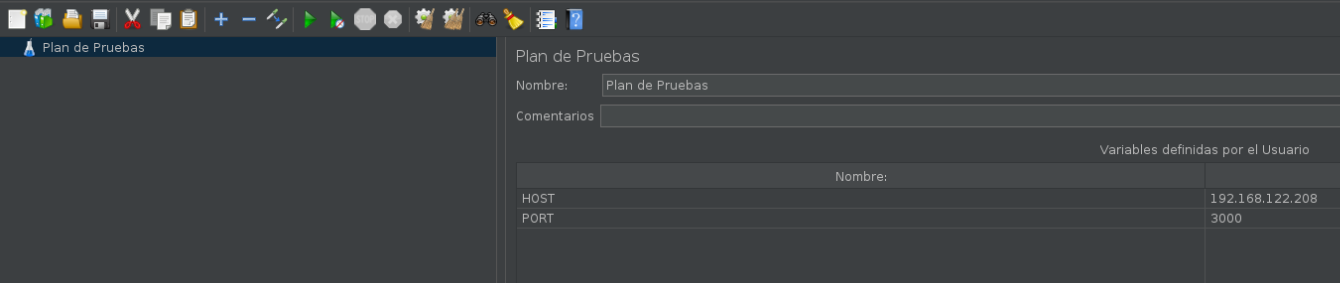
\includegraphics[scale=0.3]{JMeter/img13}
    \caption{Añadimos las variables de HOST y PORT}
\end{figure}

\newpage
\subsubsection{Hacer dos grupos de hebras distintos para alumnos y administradores para simular el acceso concurrente}

Para ello lo primero que tenemos que hacer es ver los archivos .csv que se encuentran en la carpeta iseP4JMeter/jMeter. Ahí encontraremos los archivos alumnos.csv y administradores.csv. Miramos su contenido y cogemos una cuenta de cada uno de los archivos:

\begin{figure}[H]
    \centering
    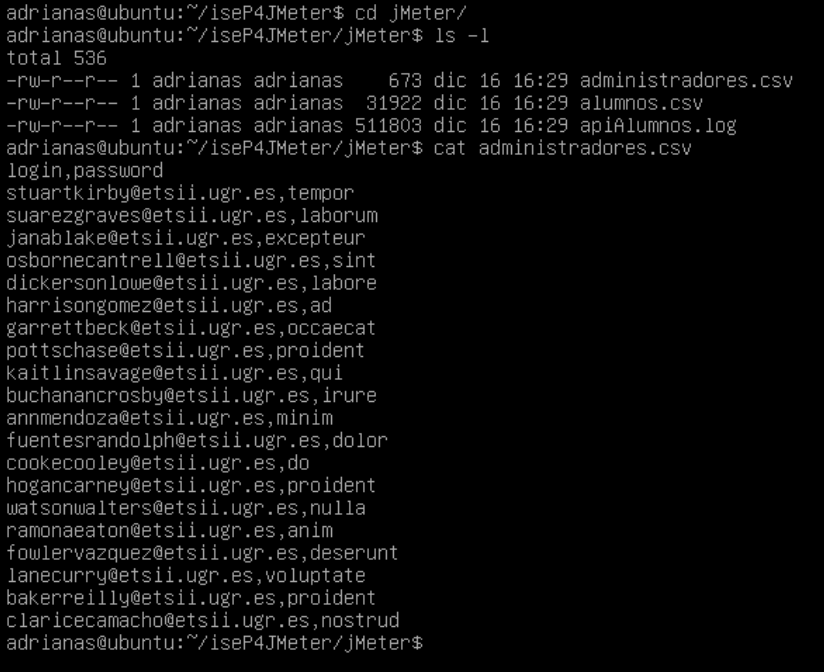
\includegraphics[scale=0.5]{JMeter/img15}
    \caption{Archivo administradores.csv}
\end{figure}

\begin{figure}[H]
    \centering
    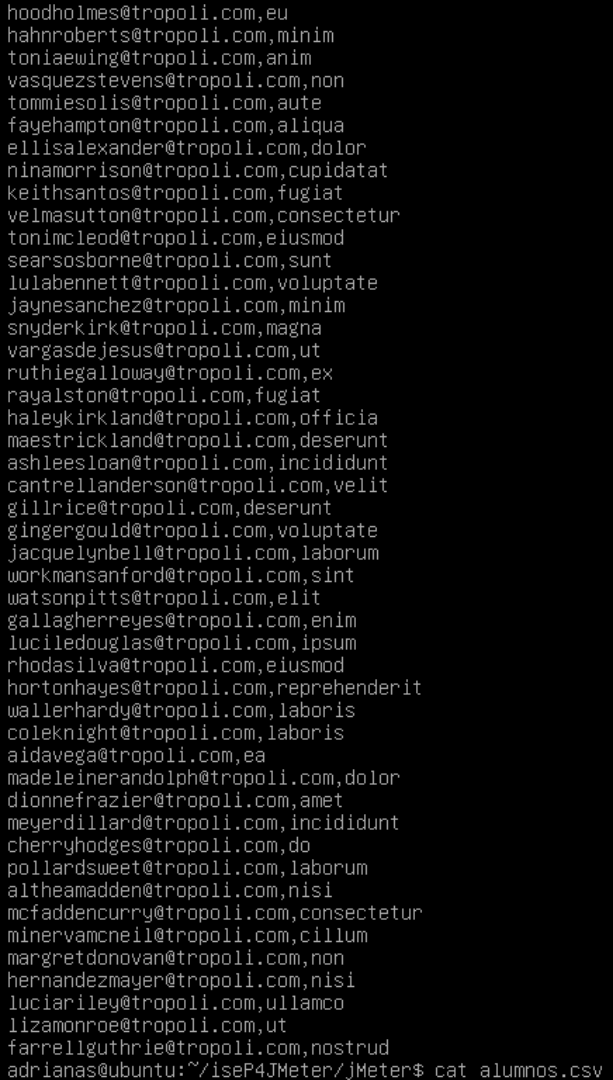
\includegraphics[scale=0.3]{JMeter/img17}
    \caption{Archivo alumnos.csv}
\end{figure}

Una vez tenemos ambas cuentas, vamos a JMeter y añadimos dos grupos de hebras que simularán el acceso de los administradores y de los alumnos.

\begin{figure}[H]
    \centering
    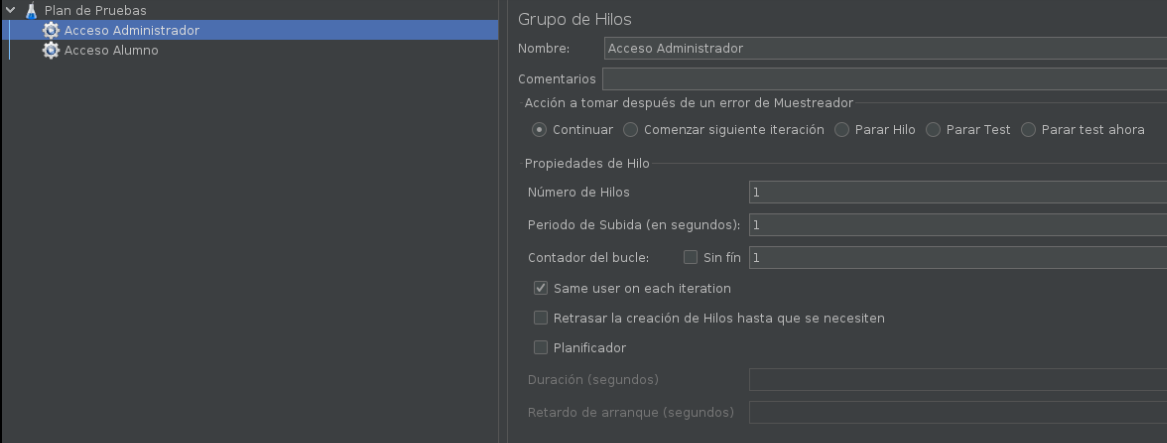
\includegraphics[scale=0.3]{JMeter/img19}
    \caption{Añadimos dos grupos de hebras}
\end{figure}

Yo he dejado todo por defecto en cada uno de los grupos de hebras. Añadimos un elemento de configuración HTTP por defecto para que en las peticiones que añadiremos a continuación tengan la IP y el Puerto configurados por defecto.

\begin{figure}[H]
    \centering
    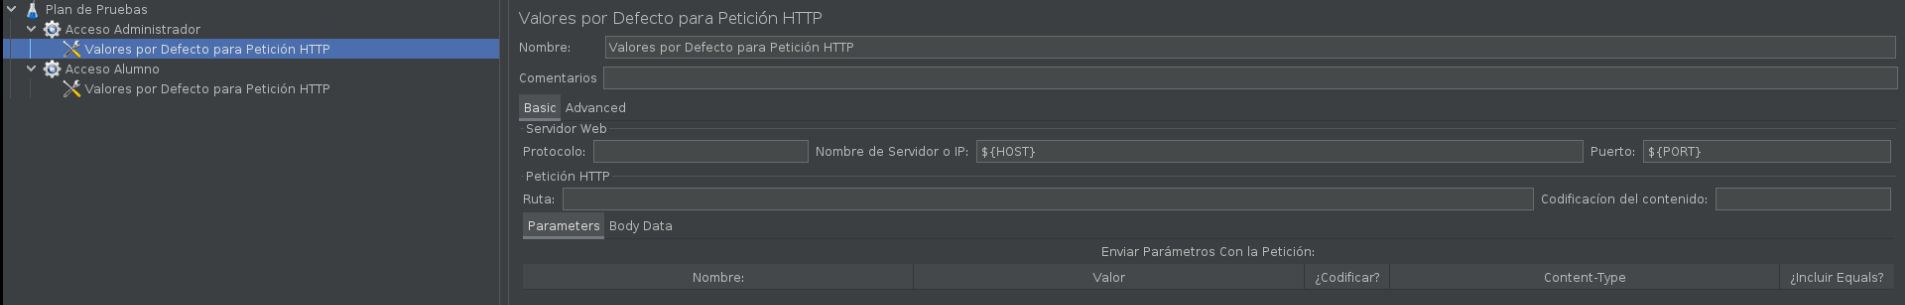
\includegraphics[scale=0.25]{JMeter/img21}
    \caption{Valores por defecto para las Peticiones HTTP}
\end{figure}

En la imagen añado un elemento a cada hebra, aunque lo más adecuado es añadirlo en general al plan de pruebas (lo hago más adelante).

Lo siguiente que tenemos que hacer es añadir una petición HTTP a cada una de las hebras para simular un login de un administrador y de un alumno:

\begin{figure}[H]
    \centering
    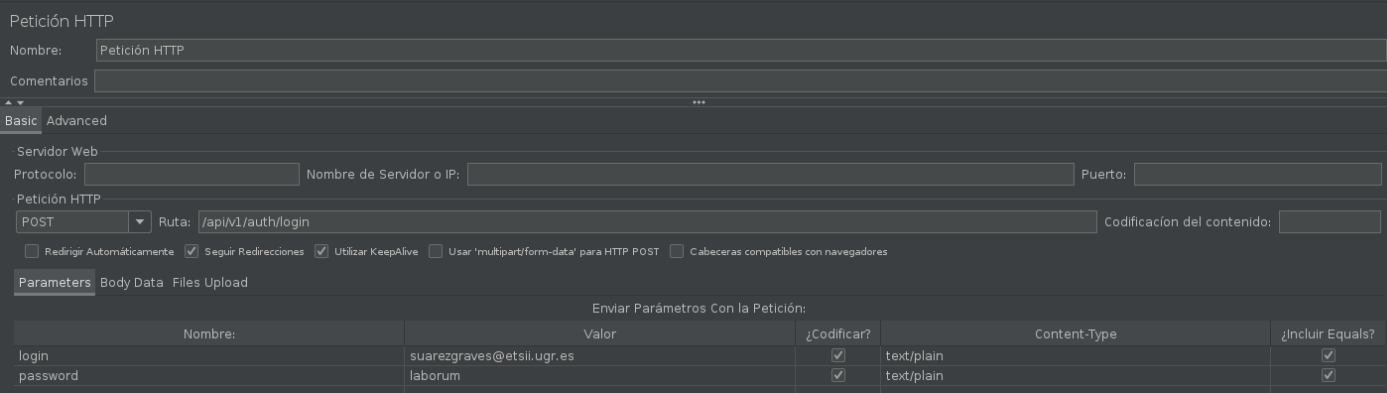
\includegraphics[scale=0.3]{JMeter/img22}
    \caption{Login de administrador}
\end{figure}

\begin{figure}[H]
    \centering
    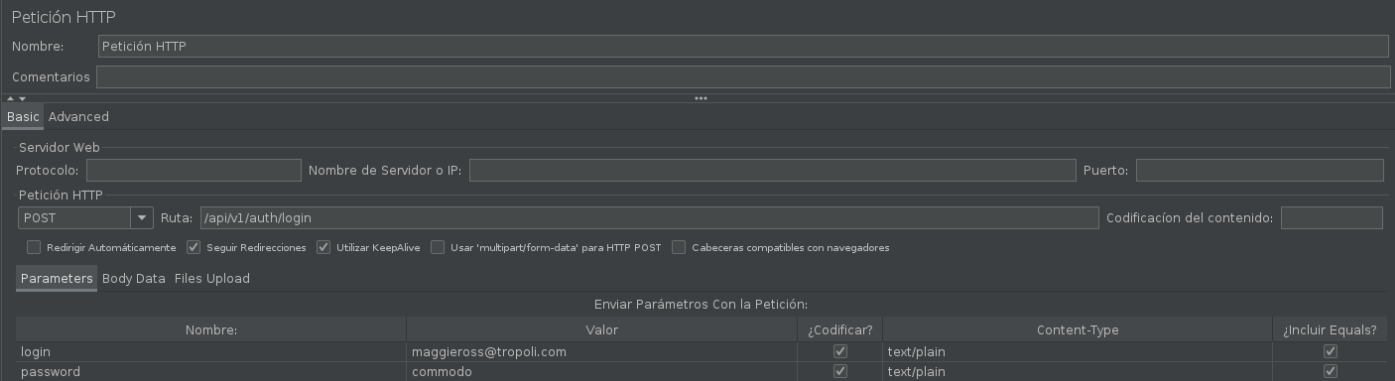
\includegraphics[scale=0.3]{JMeter/img23}
    \caption{Login de usuario}
\end{figure}

Para poder ver los resultados de ambas peticiones añadimos un árbol de resultados por defecto y ejectuamos el plan de pruebas:

\begin{figure}[H]
    \centering
    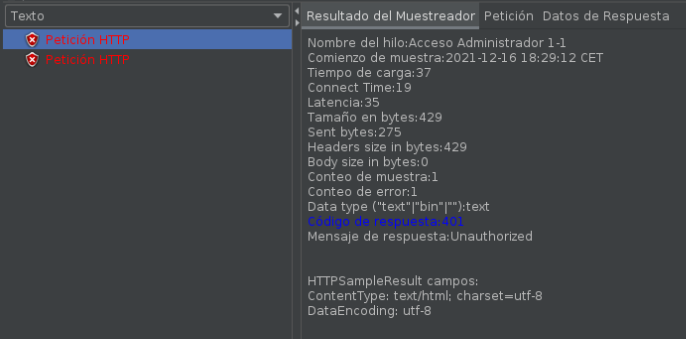
\includegraphics[scale=0.5]{JMeter/img25}
    \caption{Ejecución del plan de pruebas}
\end{figure}

Como vemos nos da error en ambos login. Esto es porque no tenemos autorización. El acceso está protegido con un BasicAuth donde el usuario es etsiiApi y la contraseña laApiDeLaETSIIDaLache. Esto aparece en la página de inicio que vimos antes.
Para solucionar este error añadimos en cada uno un gestor de autorización  HTTP con los datos ya mencionados:

\begin{figure}[H]
    \centering
    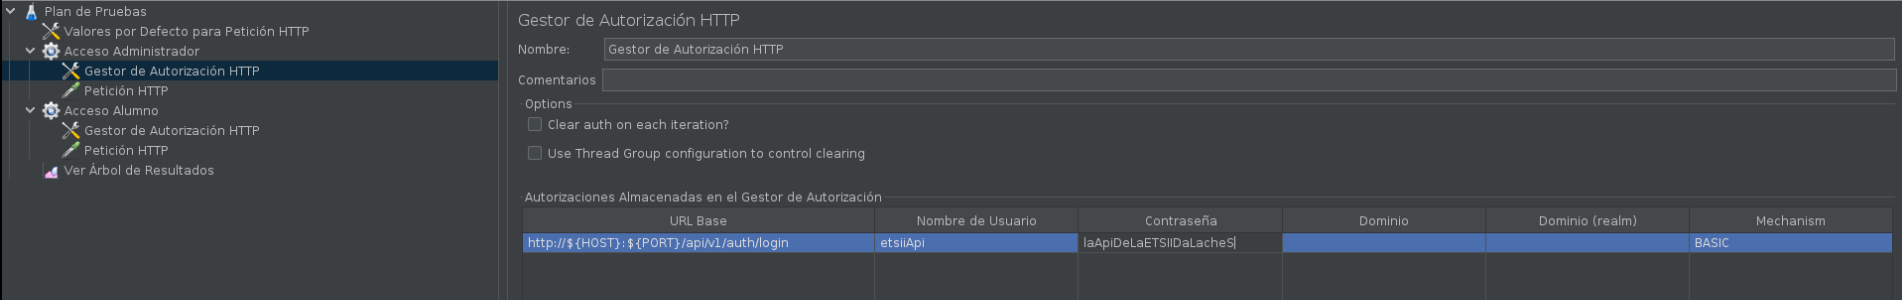
\includegraphics[scale=0.25]{JMeter/img27}
    \caption{Configuración del gestor de Autorización HTTP}
\end{figure}

\begin{figure}[H]
    \centering
    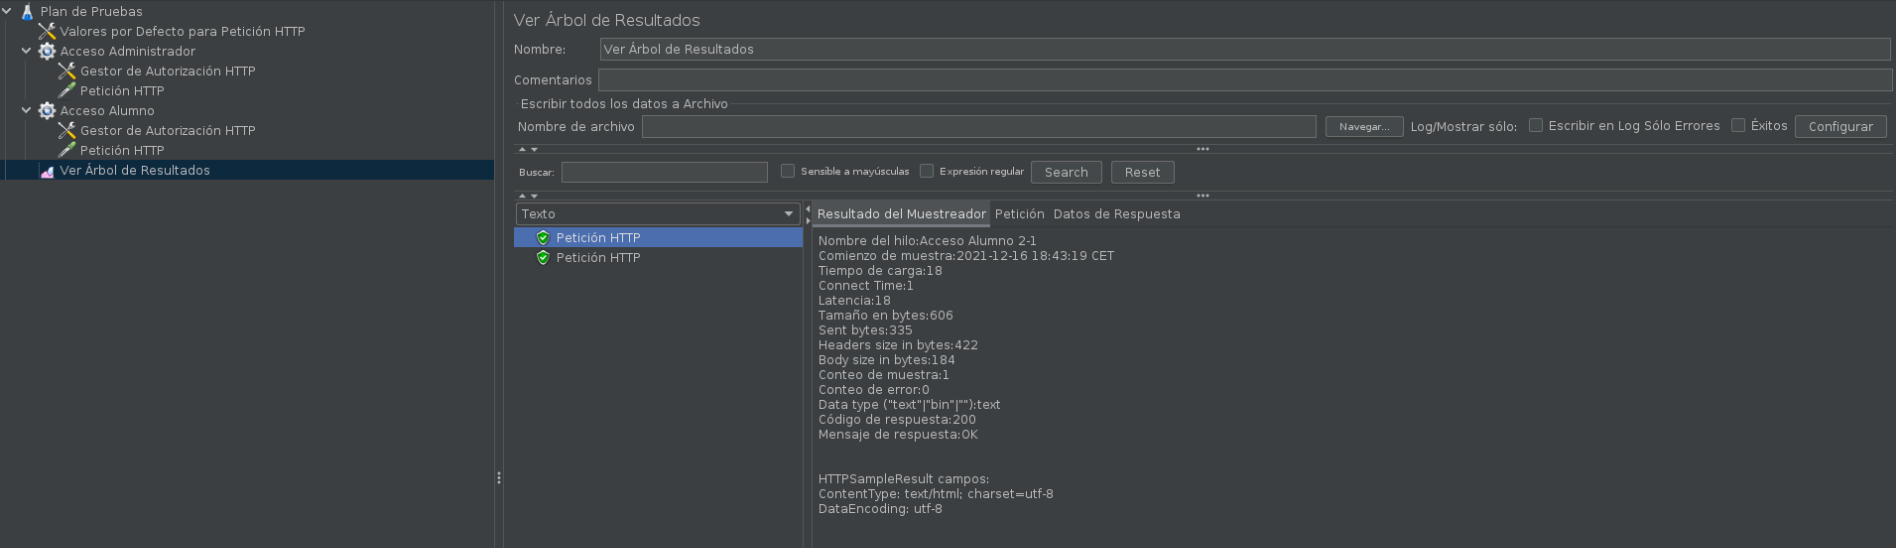
\includegraphics[scale=0.25]{JMeter/img28}
    \caption{Resultados correctos de los login}
\end{figure}

\subsubsection{Extracción del token JWT con expresiones regulares}

Para poder guardar el token que nos devuelven ambos login tenemos que crear un extractor de expresiones regulares como aparece en la siguiente imagen:

\begin{figure}[H]
    \centering
    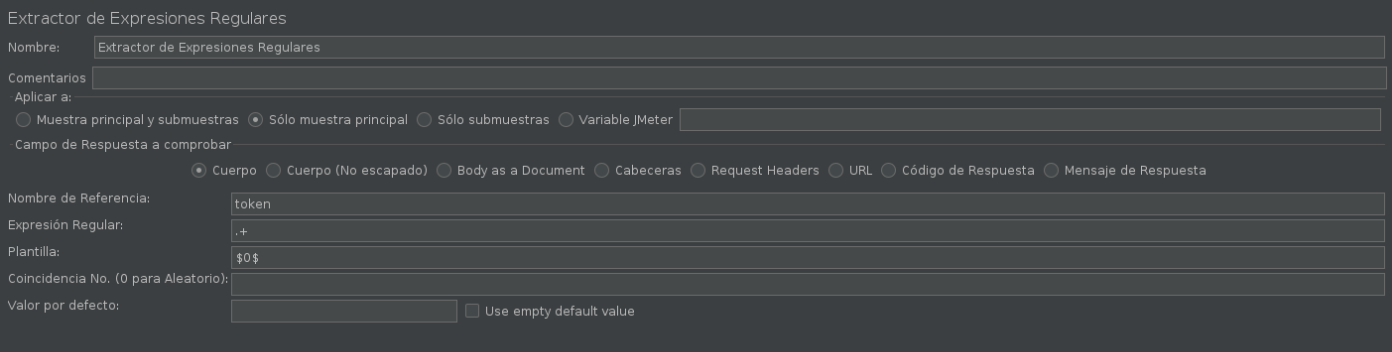
\includegraphics[scale=0.3]{JMeter/img29}
    \caption{Extractor de expresiones regulares}
\end{figure}

Para poder recibir la información usando un GET y el token hace falta que creemos otra petición HTTP donde pondremos solo la ruta del correo del alumno que queremos mostrar:

\begin{figure}[H]
    \centering
    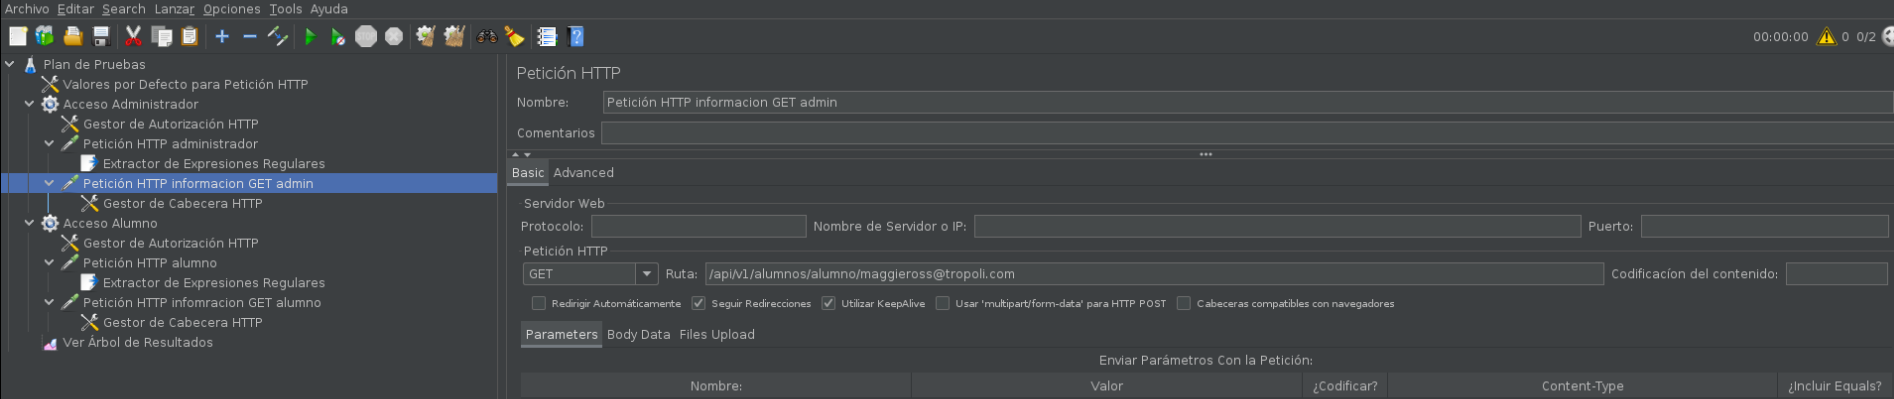
\includegraphics[scale=0.25]{JMeter/img31}
    \caption{Petición HTTP GET}
\end{figure}

También tenemos que indicar el método de seguridad usando el token que se ha recibido. Esto se hace con un gestor de cabecera HTTP, el cual se lo pondremos a la petición HTTP GET del administrador.

\begin{figure}[H]
    \centering
    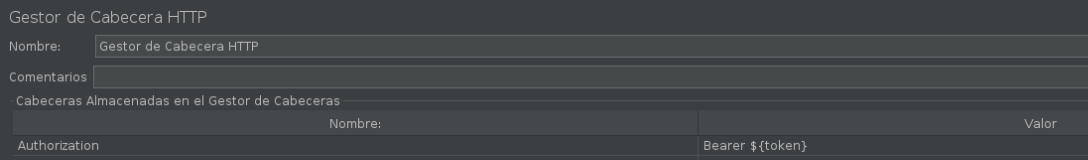
\includegraphics[scale=0.3]{JMeter/img32}
    \caption{Gestor de cabecera HTTP}
\end{figure}

Y podemos ver que funciona correctamente:

\begin{figure}[H]
    \centering
    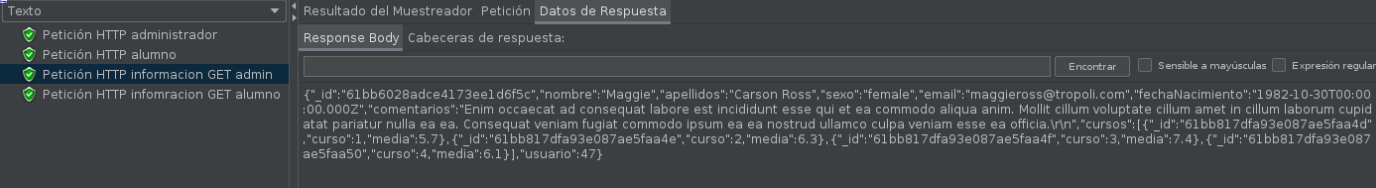
\includegraphics[scale=0.3]{JMeter/img33}
    \caption{Ejecución del plan de pruebas para comprobar si funciona}
\end{figure}

Pero para comprobar que funcione correctamente, si le indicamos un correo de un alumno en vez de un administrador pasa lo siguiente:

\begin{figure}[H]
    \centering
    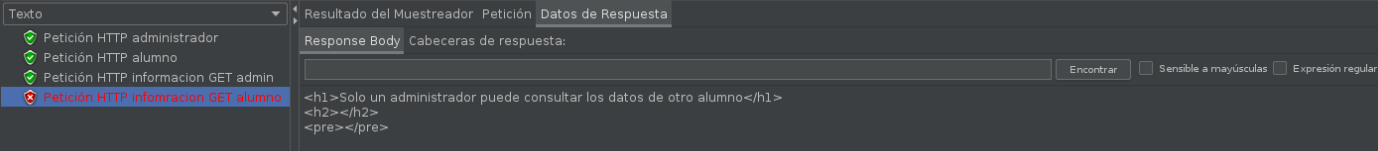
\includegraphics[scale=0.3]{JMeter/img34}
    \caption{Cambio de correo por el de un alumno}
\end{figure}

\subsubsection{Esperas aleatorias a cada grupo de hebras}

Con el objetivo de simular un entorno más realista, le añadimos a cada uno de los grupos de hebras un temporizador aleatorio Gaussiano como se ve en la siguiente imagen:

\begin{figure}[H]
    \centering
    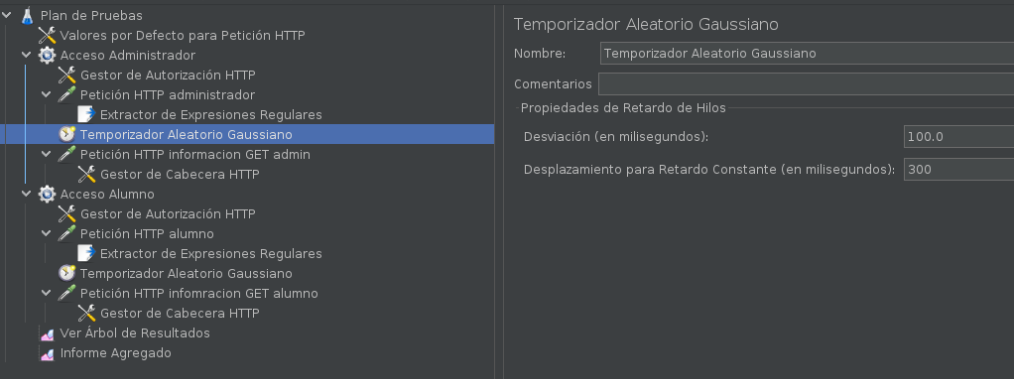
\includegraphics[scale=0.3]{JMeter/img36}
    \caption{Adición de temporizador aleatorio Gaussiano}
\end{figure}

\newpage
\subsubsection{Peticiones HTTP de los login de Alumno y Administrador}

Para ello lo primero que tenemos que hacer es añadir un elemento llamado CSV Data Set donde se accederá a los usuarios.

En la imagen hay un fallo y es que el archivo no se accede desde donde pongo. Tuve que descargar el repostorio en el host y buscar el archivo manualmente.
\begin{figure}[H]
    \centering
    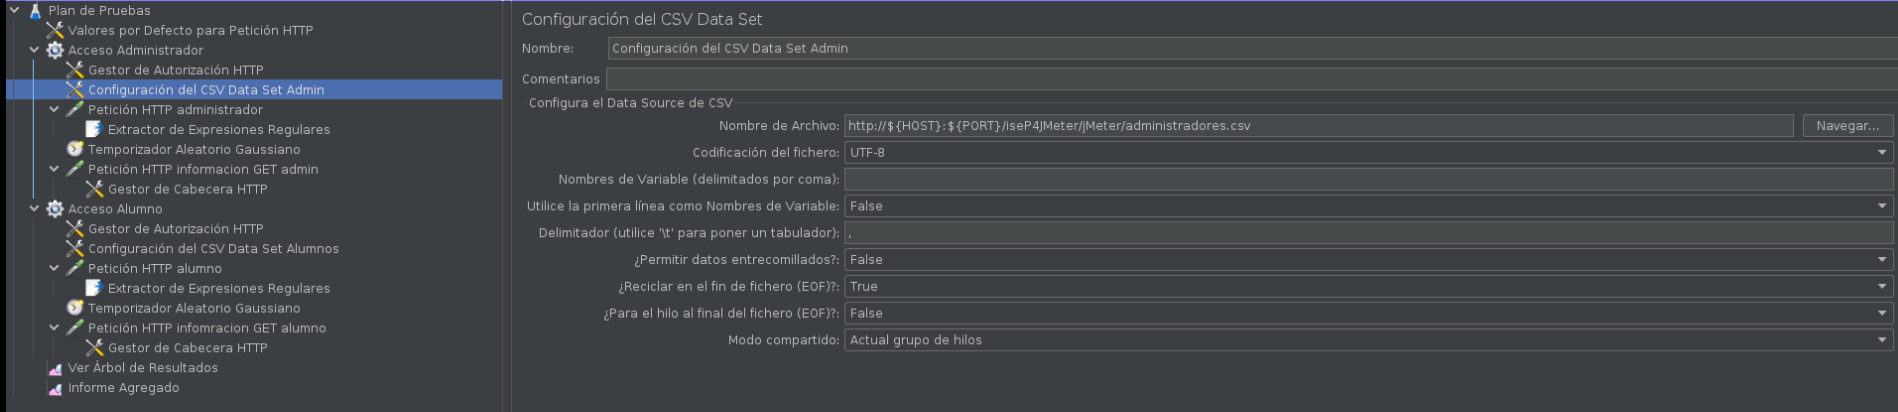
\includegraphics[scale=0.25]{JMeter/img37}
    \caption{Configuración del CSV Data Set}
\end{figure}

Y lo mismo para los alumnos. Luego hacemos una petición HTTP GET donde pondremos la siguiente información de login:

\begin{figure}[H]
    \centering
    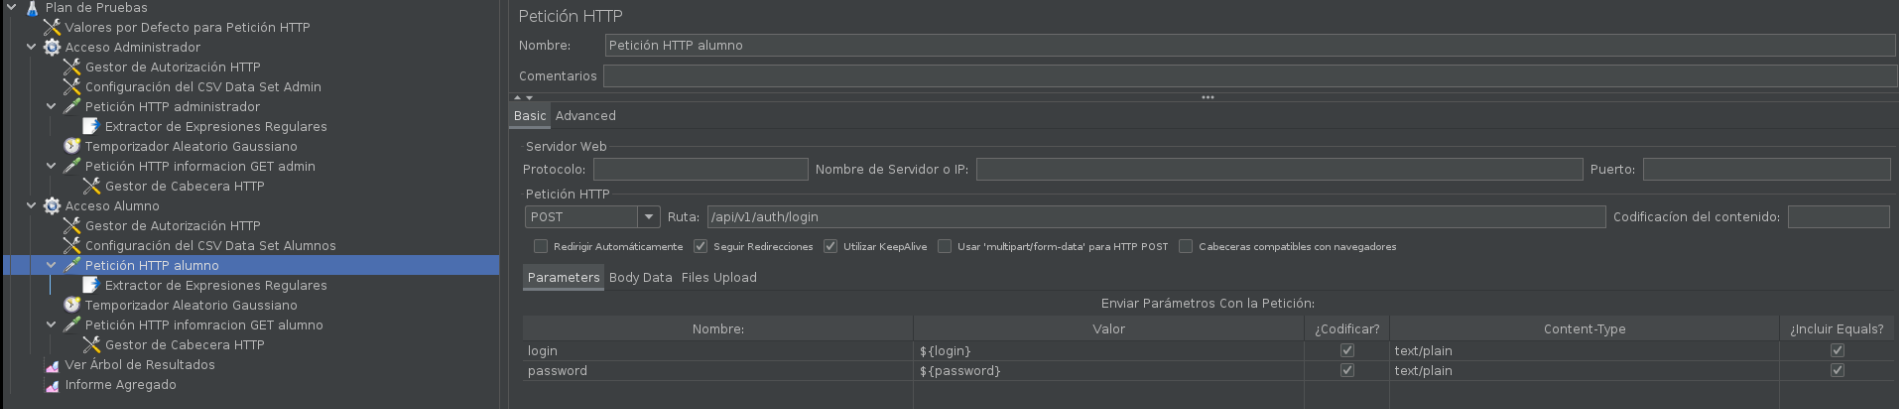
\includegraphics[scale=0.25]{JMeter/img39}
    \caption{Login de alumnos}
\end{figure}

Y al probar el plan de tests:

\begin{figure}[H]
    \centering
    \includegraphics[scale=0.3]{JMeter/img40}
    \caption{Prueba de logins}
\end{figure}

\subsubsection{Muestreo para simular el acceso de administradores}
Lo primero que tenemos que hacer es deshabilitar la petición GET del adminsitrador.

\begin{figure}[H]
    \centering
    \includegraphics[scale=0.5]{JMeter/img43}
    \caption{Deshabilitamos la peticion GET del administrador}
\end{figure}

Luego tenemos que añadir un muestreador de Acceso a Log:

\begin{figure}[H]
    \centering
    \includegraphics[scale=0.3]{JMeter/img44}
    \caption{Muestreador de Acceso a Log}
\end{figure}

Y por últmo añadimos la cabecera donde le pasamos el token de la sesión de administrador y con esto acabaríamos la práctica.
El resultado sería el siguiente:

\begin{figure}[H]
    \centering
    \includegraphics[scale=0.3]{JMeter/img45}
    \caption{Árbol de resultados final}
\end{figure}

%-------Bibliografia-----------------------------

\newpage
\section{Bibliografía}

\footnote{Instalación y configuración de Zabbix server en Rocky Linux 8 o CentOS8}
\textcolor{blue}{\url{https://techviewleo.com/install-and-configure-zabbix-server-on-rocky-linux/}}

\footnote{Instalación de Zabbix server en Rocky Linux 8 o CentOS8}
\textcolor{blue}{\url{https://www.zabbix.com/download?zabbix=5.0\&os_distribution=centos&os_version=8\&db=mysql\&ws=apache}}

\footnote{Gestión de RAID y reparación de fallos}
\textcolor{blue}{\url{https://access.redhat.com/documentation/en-\%20us/red\_hat\_enterprise\_linux/8/html/managing\_storage\_devices/managing-raid\_managing-storage-devices}}

\footnote{Instalación de Ansible en Rocky Linux 8}
\textcolor{blue}{\url{https://www.how2shout.com/linux/how-to-install-ansible-on-rocky-linux-8-or-almalinux/}}

\footnote{Conceptos básicos de Ansible}
\textcolor{blue}{\url{https://www.redhat.com/es/topics/automation/learning-ansible-tutorial}}

\footnote{Instalación de EPEL en CentOS8 o Rocky Linux 8}
\textcolor{blue}{\url{https://fedoraproject.org/wiki/EPEL/es}}

\footnote{Página del manual de linux sobre Ansible}
\textcolor{blue}{\url{https://linux.die.net/man/1/ansible}}



\end{document}
